\documentclass[12pt, titlepage]{article}
\usepackage[margin=1in]{geometry}
\usepackage[shortlabels]{enumitem}
\usepackage[utf8]{inputenc}
\usepackage{graphicx}
\usepackage{booktabs}
\usepackage{tabularx}
\usepackage{hyperref}
\hypersetup{
    colorlinks,
    citecolor=black,
    filecolor=black,
    linkcolor=red,
    urlcolor=blue
}

\usepackage[round]{natbib}

\title{SE 3XA3: Software Requirements Specification\\ GoDBMS}

\author{Team \#7, Databased
		\\ Eesha Qureshi, qureshe 
		\\ Faiq Ahmed, ahmedf46 
		\\ Kevin Kannammalil, kannammk
}

\date{February 11, 2022}

% \input{../Comments}

\begin{document}

\maketitle

\pagenumbering{roman}
\tableofcontents
\listoftables
\listoffigures

\begin{table}[h!]
\caption{\bf Revision History}
\begin{tabularx}{\textwidth}{p{3cm}p{2cm}X}
\toprule {\bf Date} & {\bf Version} & {\bf Notes}\\
\midrule
Feb 8, 2022 & 1.0 & Initial Document \\
Feb 10, 2022 & 1.1 & Finished Functional Requirements and Use Cases \\
Feb 11, 2022 & 1.2 & Completed Document \\
\bottomrule
\end{tabularx}
\end{table}

\newpage

\pagenumbering{arabic}

\noindent This document describes the requirements for the project \textbf{GoDBMS} The template for the Software Requirements Specification (SRS) is a subset of the Volere template.

\section{Project Drivers}

\subsection{The Purpose of the Project}

The purpose of this project is to build on and improve SimpleDB, to accurately demonstrate how a \textbf{DBMS} works by implementing a minimalist \textbf{DBMS} while also maintaining the ability for the \textbf{system} to perform multiple tasks at once.

\subsection{The Stakeholders}

\subsubsection{The Client}
The clients for this project are the instructional staff for SFWRENG 3XA3, as they have requested the development of this software. The staff consists of Dr. Asghar Bokhari, the professor, and his teaching assistants Veerash Palanichamy and Oluwaseun Owojaiyo. The clients will oversee the schedule for deliverables, and meet with the developers weekly to provide input and assistance as well as next steps. They will also verify that the product adheres to the requirements outlined in this document.

\subsubsection{The Customers}

The customers for this product are developers or students who are interested in learning about the fundamentals of \textbf{DBMS} and their implementation. Additionally, customers also include those who wish to use a lightweight \textbf{DBMS} due to storage costs, memory constraints or any other reason.

\subsubsection{Other Stakeholders}

Other stakeholders include the developers and quality assurance testers of the project. This consists of Eesha Qureshi, Faiq Ahmed and Kevin Kannammalil, as they will be writing, maintaining, testing and deploying all the source code for this project. Their software engineering skills are one of the resources invested in the project and it's successful development is in their best interest. Additionally, the owner of the original repository that this project is based on is also a stakeholder as they have left the code openly sourced in the interest of other developers building on or recreating it.

\subsection{Mandated Constraints}
Users of \textbf{GoDBMS} require MacOS, Windows or Linux on their machine.

\subsection{Naming Conventions and Terminology}

\begin{itemize}
    \item DBMS: database management system
    \item Concurrency/Concurrent: multiple tasks running at the same
    \item SQL: structured query language, used to describe tasks to perform in a database
    \item Query/Queries: a descriptive data request, usually written in SQL
    \item Transaction: a specific job that the database management system is instructed to perform
    \item Table: a defined structure in a database that data can be inserted into. The inserted data must abide by this structure
    \item System: in this case the system refers to our project and the overarching database management system
    \item Record: a specific entry of values in a database table
    \item Field: a column of a table in the database
    \item Schema: The structure of a table in the database, this includes all fields and constraints of the table 
\end{itemize}

\subsection{Relevant Facts and Assumptions}
\subsubsection{Assumptions}
\begin{itemize}
    \item Users have access to a computer and necessary hardware such as keypad and mouse
    \item Users have basic knowledge of SQL and queries
    \item Users have working English proficiency as other languages are not supported
    \item User has at least $\hyperlink{size}{STORAGE\_SIZE}$ space available on PC
\end{itemize}

\section{Functional Requirements}

\subsection{The Scope of the Work and the Product}

The \textbf{DBMS} being built is a simple \textbf{concurrent} database that can be used by inputting \textbf{SQL} \textbf{queries} from the command line. This \textbf{DBMS} will be implemented in a more efficient manner as compared to the original project by adding \textbf{concurrency} and the ability to handle multiple \textbf{transactions} at the same time. The project will focus on adding support for only a few primitive data types such as strings and integers and having a very basic \textbf{SQL} parser to convert the user inputs into commands the database can execute. This \textbf{SQL} parser will only support basic insert, delete and select commands with functionalities such as nested \textbf{queries} stripped.

\subsubsection{The Context of the Work}

The context of this database management \textbf{system} is going to be a command line application running on Windows, Linux, or MacOS. It will use the Go compiler to compile the program to a binary so it can natively run on the appropriate operating \textbf{system}. The user will directly interact with this application use the command line and it does not interact with other \textbf{system}s aside form the operating \textbf{system}.

\newpage

\subsubsection{Work Partitioning}

\begin{table}[h!]
    \centering
    \begin{tabular}{|l|p{4cm}|p{7cm}|}
    \hline
    \textbf{Event Name} & \textbf{Input/Output} & \textbf{Summary} \\
    \hline
    1. Create a new \textbf{table} & \textbf{Input:} \textbf{SQL} \textbf{query} \newline \textbf{Output:} Display the newly created \textbf{table} or errors & The system uses the \textbf{query} to create a \textbf{table} and display it back to the user. Alternatively error messages are displayed if the \textbf{query} is incorrect.\\
    \hline
    2. Delete a \textbf{table} & \textbf{Input:} \textbf{SQL} \textbf{query} \newline \textbf{Output:} Success message or errors & The system uses the \textbf{query} to delete a \textbf{table} and displays a message indicating success or an error.\\
    \hline
    3. List all \textbf{tables} & \textbf{Input:} \textbf{SQL} \textbf{query} \newline \textbf{Output:} A text list of all \textbf{table} names or error message & The system uses the \textbf{query} to display all stored \textbf{tables}. Alternatively error messages are displayed if the \textbf{query} is incorrect.\\
    \hline
    4. Add \textbf{record} to \textbf{table} & \textbf{Input:} \textbf{SQL} \textbf{query} \newline \textbf{Output:} Success message or errors & The system uses the \textbf{query} to store a \textbf{record} into a specified \textbf{table}. Alternatively error messages are displayed if the \textbf{query} is incorrect.\\
    \hline
    5. Modify a \textbf{record} & \textbf{Input:} \textbf{SQL} \textbf{query} \newline \textbf{Output:} A display of the modified \textbf{record} or errors & The system uses the \textbf{query} to modify a specific \textbf{record} in a \textbf{table} and displays it back to the user. Alternatively error messages are displayed if the \textbf{query} is incorrect.\\
    \hline
    6. Delete a \textbf{record} & \textbf{Input:} \textbf{SQL} \textbf{query} \newline \textbf{Output:} Success message or errors &  The system uses the \textbf{query} to delete a \textbf{record} and displays a message indicating success or an error.\\
    \hline
    7. Search for \textbf{record}s & \textbf{Input:} \textbf{SQL} \textbf{query} \newline \textbf{Output:} A display of the resulting \textbf{record}s or errors &  The system uses the \textbf{query} to find and displays all \textbf{record}s that fit the search criteria. Alternatively error messages are displayed if the \textbf{query} is incorrect.\\
    \hline
    8. Process multiple \textbf{transactions} & \textbf{Input:} \textbf{SQL} \textbf{queries} \newline \textbf{Output:} All \textbf{query} outputs &  The system takes in multiple \textbf{query} inputs and is able to process and return the correct output for all of them at the same time.\\
    \hline
    \end{tabular}
\caption{Work Partitioning Events and Summaries}
\end{table}

\newpage
\subsubsection{Individual Product Use Cases}

\begin{figure}[h!]
    \centering
    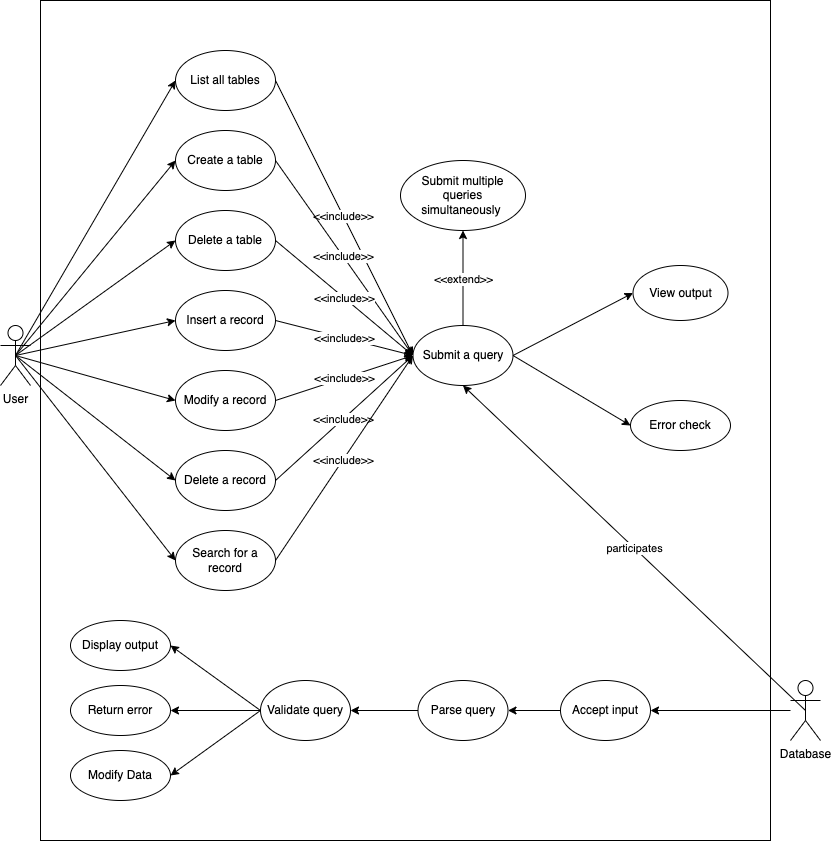
\includegraphics[scale=0.4]{images/ReqDoc.png}
    \caption{Individual Use Cases}
    \label{fig:my_label}
\end{figure}

\subsection{Functional Requirements}

\begin{enumerate}[{BE}1.]
    \item The user wants to create a \textbf{table}
    \begin{enumerate}[{FR}1.]
        \item The system must accept a command line input from the user
        \item The system must validate the syntax of the input to create a \textbf{table}
        \item The system must parse the input to identify the necessary \textbf{field}s
        \item The system must validate that the user provided a valid name for the \textbf{table} that does not already exist
        \item The system must validate that the user provided valid information about the \textbf{schema} of the \textbf{table}
        \item The system must display any errors in the input to the user
        \item The system must create a new \textbf{table} and store the \textbf{table}
        \item If the \textbf{table} is successfully created the system must display a message to the user to inform them
    \end{enumerate}
    \item The user wants to delete a \textbf{table}
    \begin{enumerate}[{FR}1.]
        \item The system must accept a command line input from the user
        \item The system must validate the syntax of the input to delete a \textbf{table}
        \item The system must parse the input to identify the necessary \textbf{field}s
        \item The system must validate that the user provided a valid name for the \textbf{table} and the \textbf{table} exists
        \item The system must display any errors in the input to the user
        \item The system must create a new delete the \textbf{table} and remove it from storage
        \item If the \textbf{table} is successfully deleted the system must display a message to the user to inform them
    \end{enumerate}
    \item The user wants to list all created \textbf{tables}
    \begin{enumerate}[{FR}1.]
        \item The \textbf{system} must accept a command line input from the user
        \item The \textbf{system} must validate the syntax of the input to list all \textbf{tables}
        \item The \textbf{system} must parse the input to identify the necessary \textbf{field}s
        \item The \textbf{system} must display any errors in the input to the user
        \item If the input is valid the \textbf{system} must display all stored \textbf{tables} and their \textbf{schema}
    \end{enumerate}
    \item The user wants to insert a \textbf{record} into a \textbf{table}
    \begin{enumerate}[{FR}1.]
        \item The \textbf{system} must accept a command line input from the user
        \item The \textbf{system} must validate the syntax of the input to insert a \textbf{record}
        \item The \textbf{system} must parse the input to identify the necessary \textbf{field}s
        \item The \textbf{system} must validate that the user provided a valid and existing \textbf{table} name to insert the \textbf{record} into
        \item The \textbf{system} must validate that the user provided a \textbf{record} that fits the \textbf{schema} of the \textbf{table} it is being inserted into
        \item The \textbf{system} must display any errors in the input to the user
        \item The \textbf{system} must create the new \textbf{record} in the \textbf{table} and add it to storage
        \item If the \textbf{record} is successfully inserted the \textbf{system} must display a message to the user to inform them
    \end{enumerate}
    \item The user wants to modify a \textbf{record} inserted into a \textbf{table}
    \begin{enumerate}[{FR}1.]
        \item The \textbf{system} must accept a command line input from the user
        \item The \textbf{system} must validate the syntax of the input to modify the \textbf{record}
        \item The \textbf{system} must parse the input to identify the necessary \textbf{field}s
        \item The \textbf{system} must validate that the user provided a valid and existing \textbf{table} name to modify the \textbf{record} from
        \item The \textbf{system} must validate that the user provided an existing, and uniquely identifiable \textbf{record} from the \textbf{table} to modify
        \item The \textbf{system} must validate that the modified \textbf{record} fits the \textbf{schema} of the \textbf{table} it is being inserted into
        \item The \textbf{system} must display any errors in the input to the user
        \item The \textbf{system} must modify the \textbf{record} in the \textbf{table} and update it in storage
        \item If the \textbf{record} is successfully updated the \textbf{system} must display a message to the user to inform them
    \end{enumerate}
    \item The user wants to delete \textbf{record}s inserted into a \textbf{table}
    \begin{enumerate}[{FR}1.]
        \item The \textbf{system} must accept a command line input from the user
        \item The \textbf{system} must validate the syntax of the input to delete the \textbf{record}s
        \item The \textbf{system} must parse the input to identify the necessary \textbf{field}s
        \item The \textbf{system} must validate that the user provided a valid and existing \textbf{table} name to delete the \textbf{record}s from
        \item The \textbf{system} must display any errors in the input to the user
        \item If any \textbf{record}s are deleted, the \textbf{system} must delete the \textbf{record}s from the \textbf{table} and remove them from storage
        \item The \textbf{system} must display all deleted \textbf{record}s to the user
    \end{enumerate}
    \item The user wants to search for \textbf{record}s inserted into \textbf{tables}
    \begin{enumerate}[{FR}1.]
        \item The \textbf{system} must accept a command line input from the user
        \item The \textbf{system} must validate the syntax of the input to search for \textbf{record}s
        \item The \textbf{system} must parse the input to identify the necessary \textbf{field}s
        \item The \textbf{system} must validate that the user provided valid and existing \textbf{table} names to search the \textbf{record}s from
        \item The \textbf{system} must display any errors in the input to the user
        \item The \textbf{system} must display all \textbf{record} from the specified \textbf{tables} that fit the user specified search criteria
    \end{enumerate}
    \item The users want to process multiple \textbf{transactions} at the same time
    \begin{enumerate}[{FR}1.]
        \item The \textbf{system} must accept and validate all inputs from the user
        \item If a \textbf{transaction} is writing to a \textbf{table} or record, the \textbf{system} must stop all \textbf{transactions} from reading from that \textbf{table} or record until the write is complete
        \item The \textbf{system} must allow multiple \textbf{transactions} to read from the same \textbf{table} or record at the same time
        \item The \textbf{system} must allow multiple \textbf{transaction} write to different \textbf{tables} or records at the same time
        \item The \textbf{system} must allow writes and reads from different \textbf{tables} or records at the same time
    \end{enumerate}
\end{enumerate}

\section{Non-functional Requirements}

\subsection{Look and Feel Requirements}
    \subsubsection{Appearance Requirements}
        \begin{enumerate}
            \item The \textbf{system} shall use a simple and minimal design
            \item The \textbf{system} should add $\hyperlink{padding}{OUTPUT\_PADDING}$ of space after each output to easily distinguish different outputs.
        \end{enumerate}
    \subsubsection{Style Requirements}
        \begin{enumerate}
            \item The \textbf{system} shall use the pre-existing styling in the command line terminal
        \end{enumerate}
\subsection{Usability and Humanity Requirements}
    \subsubsection{Ease of Use Requirements}
        \begin{enumerate}
            \item The \textbf{system} shall be easy to use for anyone with a basic understanding of a database
        \end{enumerate}
    \subsubsection{Personalization and Internationalization Requirements}
        \begin{enumerate}
            \item The \textbf{system} shall use English as the main language to communicate with the user
        \end{enumerate}
    \subsubsection{Learning Requirements}
        \begin{enumerate}
            \item The \textbf{system} shall be straightforward to use for beginners
            \item The \textbf{system} shall provide descriptive instructions to guide the user
        \end{enumerate}
    \subsubsection{Understandability and Politeness Requirements}
        N/A
    \subsubsection{Accessibility Requirements}
        \begin{enumerate}
            \item The \textbf{system} shall use the accessibility features already existing in the command line
        \end{enumerate}
\subsection{Performance Requirements}
    \subsubsection{Speed and Latency Requirements}
        \begin{enumerate}
            \item The \textbf{system} shall provide a response to the user in a reasonable time depending on the input. On average the \textbf{transactions} should respond within $\hyperlink{time}{RESPONSE\_TIME}$.
        \end{enumerate}
    \subsubsection{Safety-Critical Requirements}
        N/A
    \subsubsection{Precision or Accuracy Requirements}
        \begin{enumerate}
            \item The \textbf{system} shall not round any of the outputs to preserve the accuracy of the data
        \end{enumerate}
    \subsubsection{Reliability and Availability Requirements}
        N/A
    \subsubsection{Robustness or Fault-Tolerance Requirements}
        N/A
    \subsubsection{Capacity Requirements}
        \begin{enumerate}
            \item The \textbf{system} will store all the data locally on the user's device
        \end{enumerate}
    \subsubsection{Scalability or Extensibility Requirements}
        \begin{enumerate}
            \item The \textbf{system} can be vertically scaled with the hardware of the environment it is running in
        \end{enumerate}
    \subsubsection{Longevity Requirements}
        \begin{enumerate}
            \item The \textbf{system} shall be developed to be easily maintainable in the long term
        \end{enumerate}
\subsection{Operational and Environmental Requirements}
    \subsubsection{Expected Physical Environment}
        \begin{enumerate}
            \item The \textbf{system} is not dependent on an internet connection to work
            \item The \textbf{system} should be used on a computer that can run the command line
        \end{enumerate}
    \subsubsection{Requirements for Interfacing with Adjacent Systems}
        N/A
    \subsubsection{Productization Requirements}
        N/A
    \subsubsection{Release Requirements}
        \begin{enumerate}
            \item The \textbf{system} will have it's final iteration and release on April 12th 2021
        \end{enumerate}
\subsection{Maintainability and Support Requirements}
    \subsubsection{Maintenance Requirements}
        \begin{enumerate}
            \item The \textbf{system} will be fully documented on how to use it
            \item The \textbf{system} will have diagrams regarding the architecture and code
            \item The \textbf{system} will use consistent styling
        \end{enumerate}
    \subsubsection{Supportability Requirements}
        \begin{enumerate}
            \item The \textbf{system} will be open source
            \item The \textbf{system} is supported to run on Windows, MacOS and Linux devices
        \end{enumerate}
    \subsubsection{Adaptability Requirements}
        N/A

\subsection{Security Requirements}
    \subsubsection{Access Requirements}
        \begin{enumerate}
            \item The \textbf{system}'s code will only be view-able to the public through the git repository. 
            \item The \textbf{system} restricts it's editing privileges for the code only to the maintainers. 
        \end{enumerate}
    \subsubsection{Integrity Requirements}
        N/A
    \subsubsection{Privacy Requirements}
        \begin{enumerate}
            \item The \textbf{system} shall not collect any personal information of the users 
            \item The \textbf{system} will not require the user to create an account
        \end{enumerate}
    \subsubsection{Audit Requirements}
        N/A
    \subsubsection{Immunity Requirements}
        N/A

\subsection{Cultural Requirements}
    N/A

\subsection{Legal Requirements}
    \subsubsection{Compliance Requirements}
        \begin{enumerate}
            \item The \textbf{system} is not accountable for the legality of the data that is being stored
            \item The \textbf{system} is not responsible for the loss of any data
            \item The \textbf{system} is meant for learning purposes only and not for use in production
            \item The \textbf{system} will not use any copyrighted information
        \end{enumerate}
        
    \subsubsection{Standards Requirements}
        \begin{enumerate}
            \item The \textbf{system} shall follow the IEEE standards
        \end{enumerate}
\subsection{Health and Safety Requirements}
    \begin{enumerate}
        \item The \textbf{system} will not have any health and safety concerns for users 
    \end{enumerate}
This section is not in the original Volere template, but health and safety are
issues that should be considered for every engineering project.

\section{Project Issues}

\subsection{Open Issues}

There are no open issue in the actual SimpleDB repository and the last commit was in 2019. The original implementation is correct and functional. Since the original implementation is written in Java, it requires the Java Runtime Environment to function. Thus, only hardware that has the JRE installed can run the original implementation of this project.

\subsection{Off-the-Shelf Solutions}

There are various off the shelf solutions to a \textbf{DBMS} that are well documented, correct, easy to use, and open source. However, to improve productivity and functionality of the software, many additional features such as support for multiple different data types and custom functions tend to be added into these off-the-shelf solutions. On the other hand many of existing simplistic \textbf{DBMS} tend to not include features such as \textbf{concurrency} or \textbf{SQL} parsing in them.\\

\noindent Though the code from the original repository can not be copied since we are implementing our \textbf{system} in a different language, many of the concepts and implementations can be referenced in our project.

\subsection{New Problems}

Since the project will not be compiled to a binary using Go compiler, the \textbf{system} would no longer need the Java Runtime Environment for the application to function as compared to the original project. However to be able to initially install the project, the Go compiler would need to be installed on the environment. It may be difficult for the user to install and compile from source code on their own.

\subsection{Tasks}

The tasks and schedule for this project can be found in our \href{https://gitlab.cas.mcmaster.ca/ahmedf46/GoDBMS_L01_GRP07/-/blob/main/ProjectSchedule/GanttChart.pdf}{Gantt Chart}

\subsection{Migration to the New Product}

Not applicable, since GoDBMS will be built from scratch and independent of the original project.

\subsection{Risks}

There are very few risks with this project. It runs independently on an operating \textbf{system} and is only meant to be used as learning tool rather than a production database. This project may have risks of using up excessive amounts of resources on the operating \textbf{system} which may effect the performance of the operating system. These risks can be minimized by testing and ensuring the correctness of the code.

\subsection{Costs}

There are no monetary costs associated with this project. All software used in the development and installation of this project is open source and free to use.

\subsection{User Documentation and Training}

Very minimal documentation is required for this project. Since we are removing certain features from the \textbf{SQL} parsing though, documentation should be provided to the user through the command line interface on which \textbf{SQL} features are available in this \textbf{DBMS}.\\

\noindent The user will need to be trained in the basics of \textbf{SQL} to be able to use this \textbf{DBMS}. There are various existing resources to learn about \textbf{SQL} already available. The user can given a link to the \href{https://www.w3schools.com/sql/}{W3 SQL Tutorial} to be trained in \textbf{SQL}.

\subsection{Waiting Room}

The following features can be added in future release to improve the functionality of the \textbf{DBMS} while maintaining its simplicity.

\begin{enumerate}[{FR}1.]
    \item Nested \textbf{SQL} \textbf{queries}
    \item Graphical User Interface to view and modify the database
\end{enumerate}

\subsection{Ideas for Solutions}

A simple shell script or batch script can be included to assist users in the installation of this project, which includes installing the Go compiler and compiling the project to a binary.

\bibliographystyle{plainnat}

\bibliography{SRS}

\newpage

\section{Appendix}

This section has been added to the Volere template.  This is where you can place
additional information.

\subsection{Symbolic Parameters}

The definition of the requirements will likely call for SYMBOLIC\_CONSTANTS.
Their values are defined in this section for easy maintenance.\\

\noindent $\hypertarget{padding}{OUTPUT\_PADDING}$ = 20px \\
\noindent $\hypertarget{time}{RESPONSE\_TIME}$ = 5 seconds \\
\noindent $\hypertarget{size}{STORAGE\_SIZE}$ = 1 GB\\

\end{document}
